\section{Results}
\label{sec:results}

\subsection{Patient networks are made of many tight groups}

Table~\ref{tab:networks} gives the main measures and Figure~\ref{fig:pictures} shows the three long-stay networks. The honest networks are very different from random ones. Their triangle rate is about 0.5, against 0.001--0.002 in the random networks: patients with similar histories form tight triangles. Paths are longer than in the random networks (9.4 against 5.3 steps for long stay), because the network is a chain of local groups rather than one well-mixed whole. Community structure is very strong (modularity 0.94 and 0.92), with hundreds of small groups.

\begin{table*}[!t]
\centering
\caption{Network measures for the honest, cheating, and random networks. Random values are averages over 10 rewirings.}
\label{tab:networks}
\small
\begin{tabular}{lrrrrrr}
\toprule
 & \multicolumn{3}{c}{Long stay} & \multicolumn{3}{c}{New high blood pressure} \\
\cmidrule(lr){2-4}\cmidrule(lr){5-7}
Measure & Honest & Cheating & Random & Honest & Cheating & Random \\
\midrule
Connections                 & 18,581 & 17,478 & 18,581 & 9,787 & 8,883 & 9,787 \\
Stays in largest group      & 88.2\% & 62.8\% & 95.6\% & 88.0\% & 74.6\% & 95.1\% \\
Triangle rate               & 0.494 & 0.660 & 0.001 & 0.479 & 0.589 & 0.002 \\
Average path (steps)        & 9.4 & 11.5 & 5.3 & 8.1 & 9.4 & 4.8 \\
Modularity                  & 0.938 & 0.977 & 0.546 & 0.922 & 0.958 & 0.540 \\
Homophily                   & 0.211 & 0.201 & 0.010 & 0.226 & 0.263 & 0.002 \\
Homophily, different patients & 0.239 & 0.228 & 0.010 & 0.115 & 0.154 & 0.002 \\
Same-patient connections    & 37.8\% & 39.3\% & 0.1\% & 29.5\% & 29.5\% & 0.2\% \\
Explained by communities    & 0.109 & 0.130 & 0.008 & 0.074 & 0.136 & 0.010 \\
\bottomrule
\end{tabular}
\end{table*}

\begin{figure*}[!t]
\centering
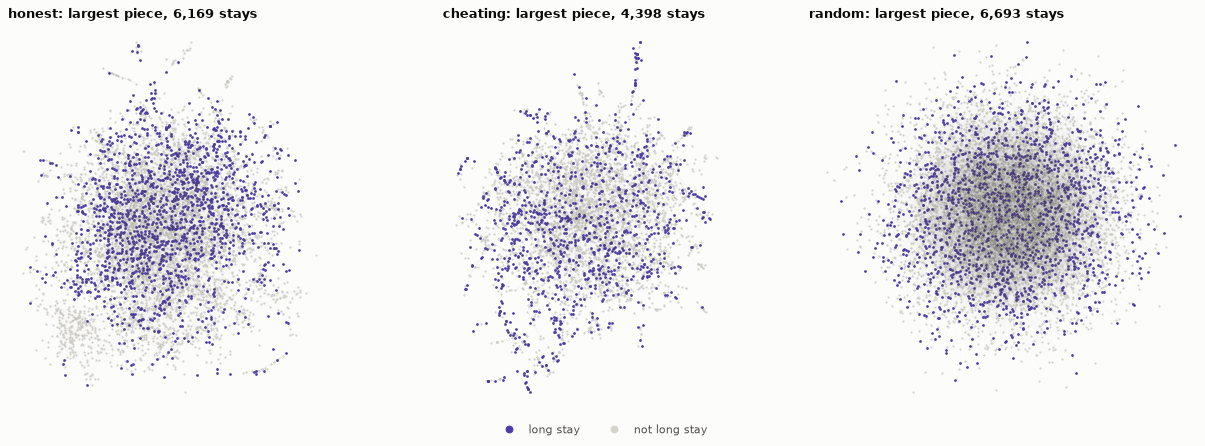
\includegraphics[width=\textwidth]{02_network_pictures.png}
\caption{The honest, cheating, and random long-stay networks (largest connected group; positions are for display only). The honest and cheating networks break into many small, tight clusters; the random network is one tangled ball.}
\label{fig:pictures}
\end{figure*}

\subsection{Connected stays share outcomes}

In both honest networks, connected stays share outcomes far more than chance: homophily is 0.21 for long stay and 0.23 for high blood pressure, against about 0.01 in the random networks. In plain numbers, 40\% of the connections of a long stay lead to another long stay, although only 25\% of all stays are long (24\% in the random network). For high blood pressure the figures are 32\% against a base rate of 13\%.

The communities show the same pattern (Figure~\ref{fig:groups}). Some have almost no long stays and others have more than half, whereas random communities all stay close to the overall rate. Community membership explains about 11\% of the variation in long stay and 7\% in high blood pressure, against 1\% by chance.

\begin{figure*}[!t]
\centering
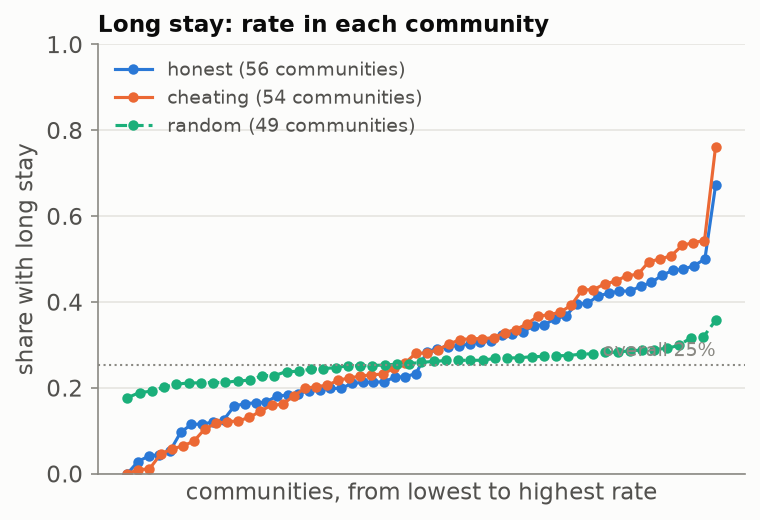
\includegraphics[width=0.49\textwidth]{02_group_outcome_rates.png}\hfill
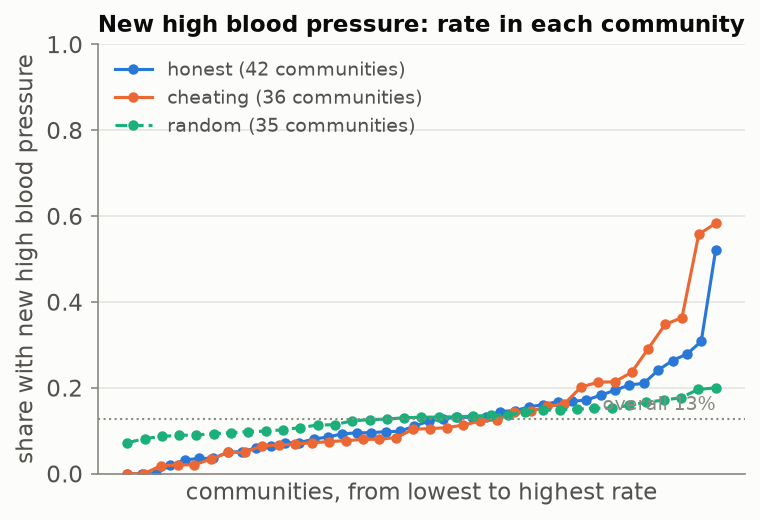
\includegraphics[width=0.49\textwidth]{03_group_outcome_rates.png}
\caption{Outcome rate in each community with at least 20 stays, sorted from lowest to highest. Honest and cheating communities range from almost no positives to well above the overall rate (dotted line); random communities all sit near it.}
\label{fig:groups}
\end{figure*}

\paragraph{Connections between stays of the same patient.} About a third of connections join two stays of the same patient (37.8\% for long stay, 29.5\% for high blood pressure). For long stay these agree on the outcome 68.5\% of the time, close to the 62\% expected if outcomes were drawn at random, and removing them slightly \emph{raises} homophily (0.211 to 0.239). For high blood pressure they agree 94.9\% of the time against 77.7\% expected, and removing them halves homophily (0.226 to 0.115). So for long stay the pattern comes from different patients with similar histories, while for high blood pressure much of it comes from the same patient appearing several times.

\paragraph{Being central does not mean being sick.} How connected or central a stay is says almost nothing about its outcome: centrality scores separate positive from negative stays no better than a coin flip (AUROC 0.47--0.58).

\subsection{Leakage depends on the question}

Figure~\ref{fig:both} compares the honest and cheating networks for both questions.

For \textbf{long stay}, adding the future barely matters for outcomes: homophily even drops slightly (0.211 to 0.201). The network's \emph{shape} does change. With twice as many diagnoses per stay it breaks into more pieces, and only 62.8\% of stays remain in the largest group. The strongest single giveaway in the future record is pleural effusion (fluid around the lungs), present for 63\% of long stays and 37\% of the others, but it does not reorganise the network. The reason is simple: ``a stay of 7 days or more'' is not itself a diagnosis, so the future record does not contain the answer.

For \textbf{new high blood pressure}, leakage is clearly visible. Homophily rises from 0.226 to 0.263, and among connections between different patients from 0.115 to 0.154, an increase of about a third. Community membership explains almost twice as much of the outcome (7.4\% to 13.6\%). Here the future record does contain the answer: by definition, every positive stay's later record includes the hypertension diagnosis, against only 13\% of negative stays (those diagnosed more than a year later). In the honest record, no single diagnosis differs by more than 11 percentage points between the two groups. This is a property of how the task is defined, not an early warning sign a hospital could use.

\begin{figure*}[!t]
\centering
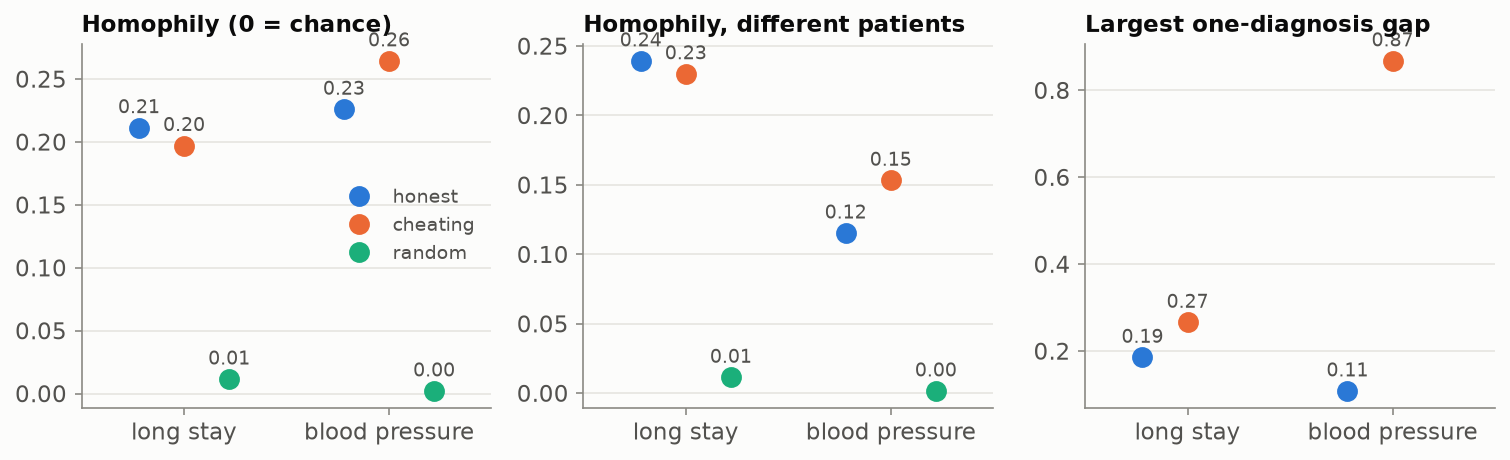
\includegraphics[width=\textwidth]{06_both_questions.png}
\caption{Honest (blue), cheating (orange), and random (green) networks for both questions. Left: homophily. Middle: homophily using only connections between different patients. Right: the largest gap between positive and negative stays in how often a single diagnosis appears. Cheating changes little for long stay but clearly helps for high blood pressure, where the diagnosis being predicted appears in the future record.}
\label{fig:both}
\end{figure*}

Why does homophily rise only modestly when the answer is in the record? Because the weighting gives very little weight to diagnoses that many patients share, and hypertension is one of the most common diagnoses in the data. Figure~\ref{fig:cheat-htn} shows the effect connection by connection: leakage can be present and still look small in a single summary number.

\begin{figure*}[!t]
\centering
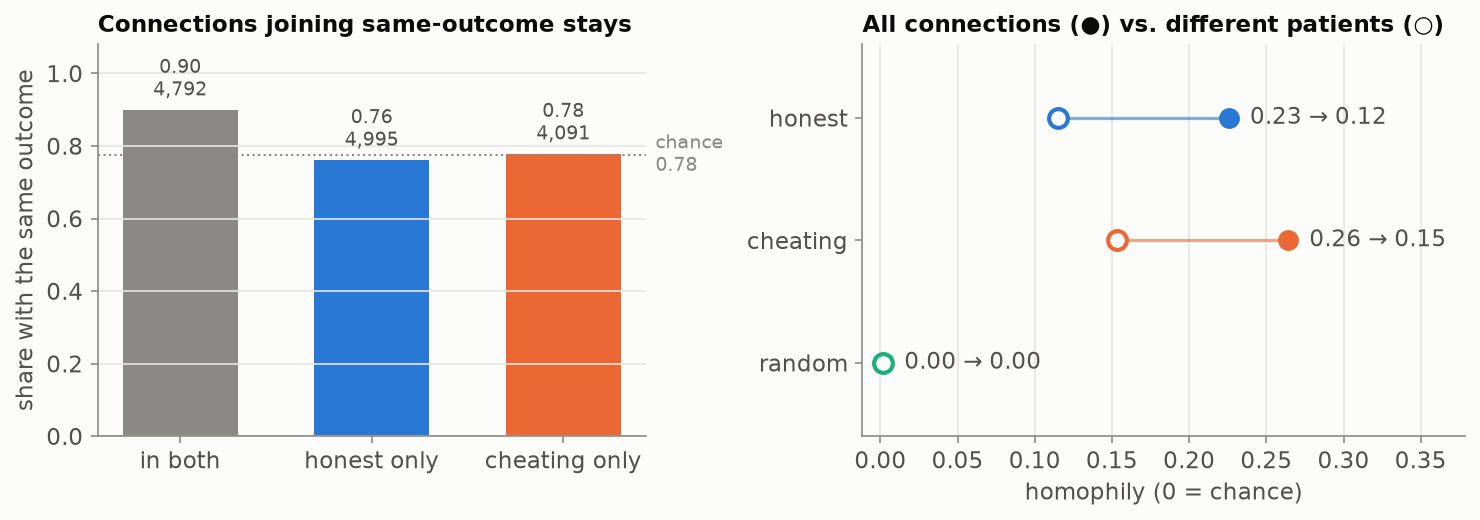
\includegraphics[width=0.9\textwidth]{03_what_cheating_changes.png}
\caption{New high blood pressure. Left: share of connections joining two stays with the same outcome, for connections found in both networks, only in the honest network, and only in the cheating network (dotted line: chance; numbers below the share are connection counts). Right: homophily with all connections (filled) and with only connections between different patients (open).}
\label{fig:cheat-htn}
\end{figure*}

\subsection{Billing codes can split the data in two}
\label{sec:robust}

If we build the patient networks from raw billing codes instead of standardised codes, stays from before and after the 2015 switch almost never connect: only 1 of 18,693 long-stay connections and 5 of 9,892 high-blood-pressure connections cross the switch. (These billing-code networks have slightly different numbers of connections than the main ones.) With standardised codes, 3.0\% and 4.1\% of connections cross it. To check that the switch does not explain our outcome results, we shuffled outcomes separately among stays before and after 2015, which keeps any before/after difference but removes everything else. Homophily falls to 0.004 and 0.014, against 0.211 and 0.226 in reality, so the switch accounts for at most about 2\% and 6\% of the observed homophily. The leakage results also hold on billing codes: cheating raises high-blood-pressure homophily from 0.226 to 0.282 and leaves long stay unchanged (0.209 against 0.205).

\subsection{Diseases that follow each other form families}

The diagnosis network makes the billing-code problem even clearer. Built on raw billing codes, it has 134 diagnoses and 584 connections, but it falls apart into one piece of 69 codes, all ICD-10, and one of 47 codes, all ICD-9, with no connection between them (Figure~\ref{fig:rawtree}). Its first split separates old codes from new ones: a change in paperwork, not in medicine.

\begin{figure*}[!t]
\centering
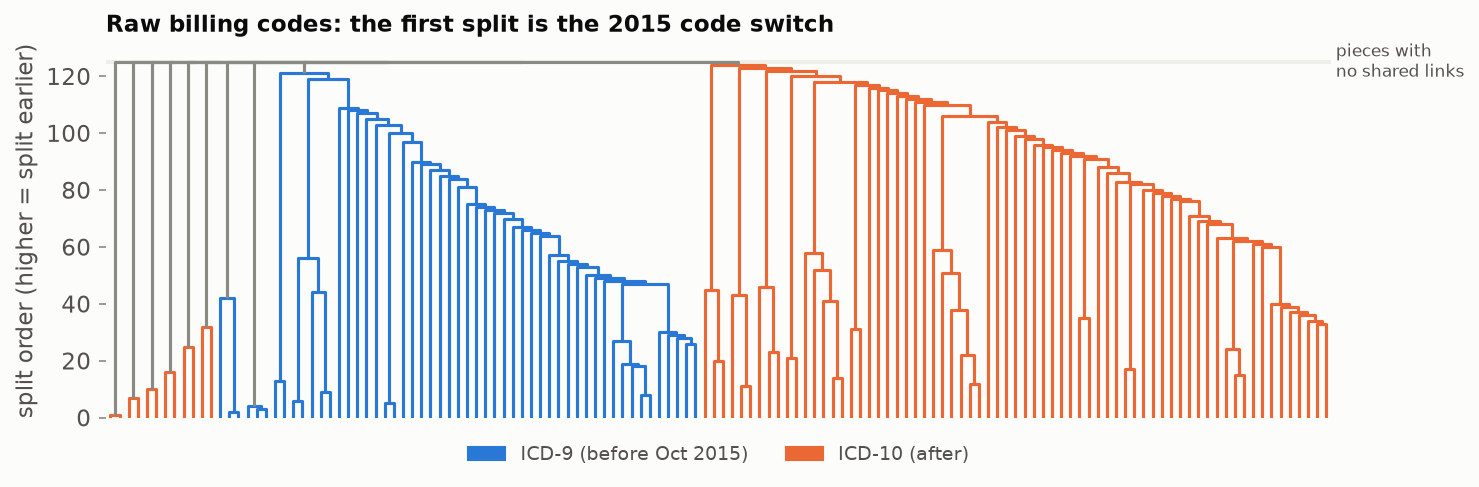
\includegraphics[width=\textwidth]{04_raw_codes_tree.png}
\caption{Tree of splits for the diagnosis network built on raw billing codes. The top split separates ICD-9 from ICD-10 codes.}
\label{fig:rawtree}
\end{figure*}

With standardised codes the network has 79 diagnoses and 142 connections, with one main piece of 60 diagnoses. The best cut of the Girvan--Newman tree gives 13 groups (modularity 0.57), similar to what Louvain finds (adjusted Rand index 0.65, where 1 means identical groups). The largest groups are clinically recognisable (Figure~\ref{fig:families}):
\begin{itemize}
  \item \textbf{Lung and breathing failure} (19 diagnoses): acute respiratory failure, pleural effusion, pneumonia, and collapsed lung tissue (atelectasis).
  \item \textbf{Sepsis and kidney failure} (18): sepsis, septic shock, bacteria in the blood, and acute kidney failure.
  \item \textbf{Heart failure} (14): congestive heart failure, cardiomyopathy, and heart disease caused by high blood pressure.
  \item Smaller groups: irregular heartbeat (5), pregnancy (4), and type 2 diabetes complications (4).
\end{itemize}
A few small pairs are the same condition recorded two ways, such as ``vomiting'' and ``nausea and vomiting''; these reflect recording habits rather than disease progression.

\begin{figure*}[p]
\centering
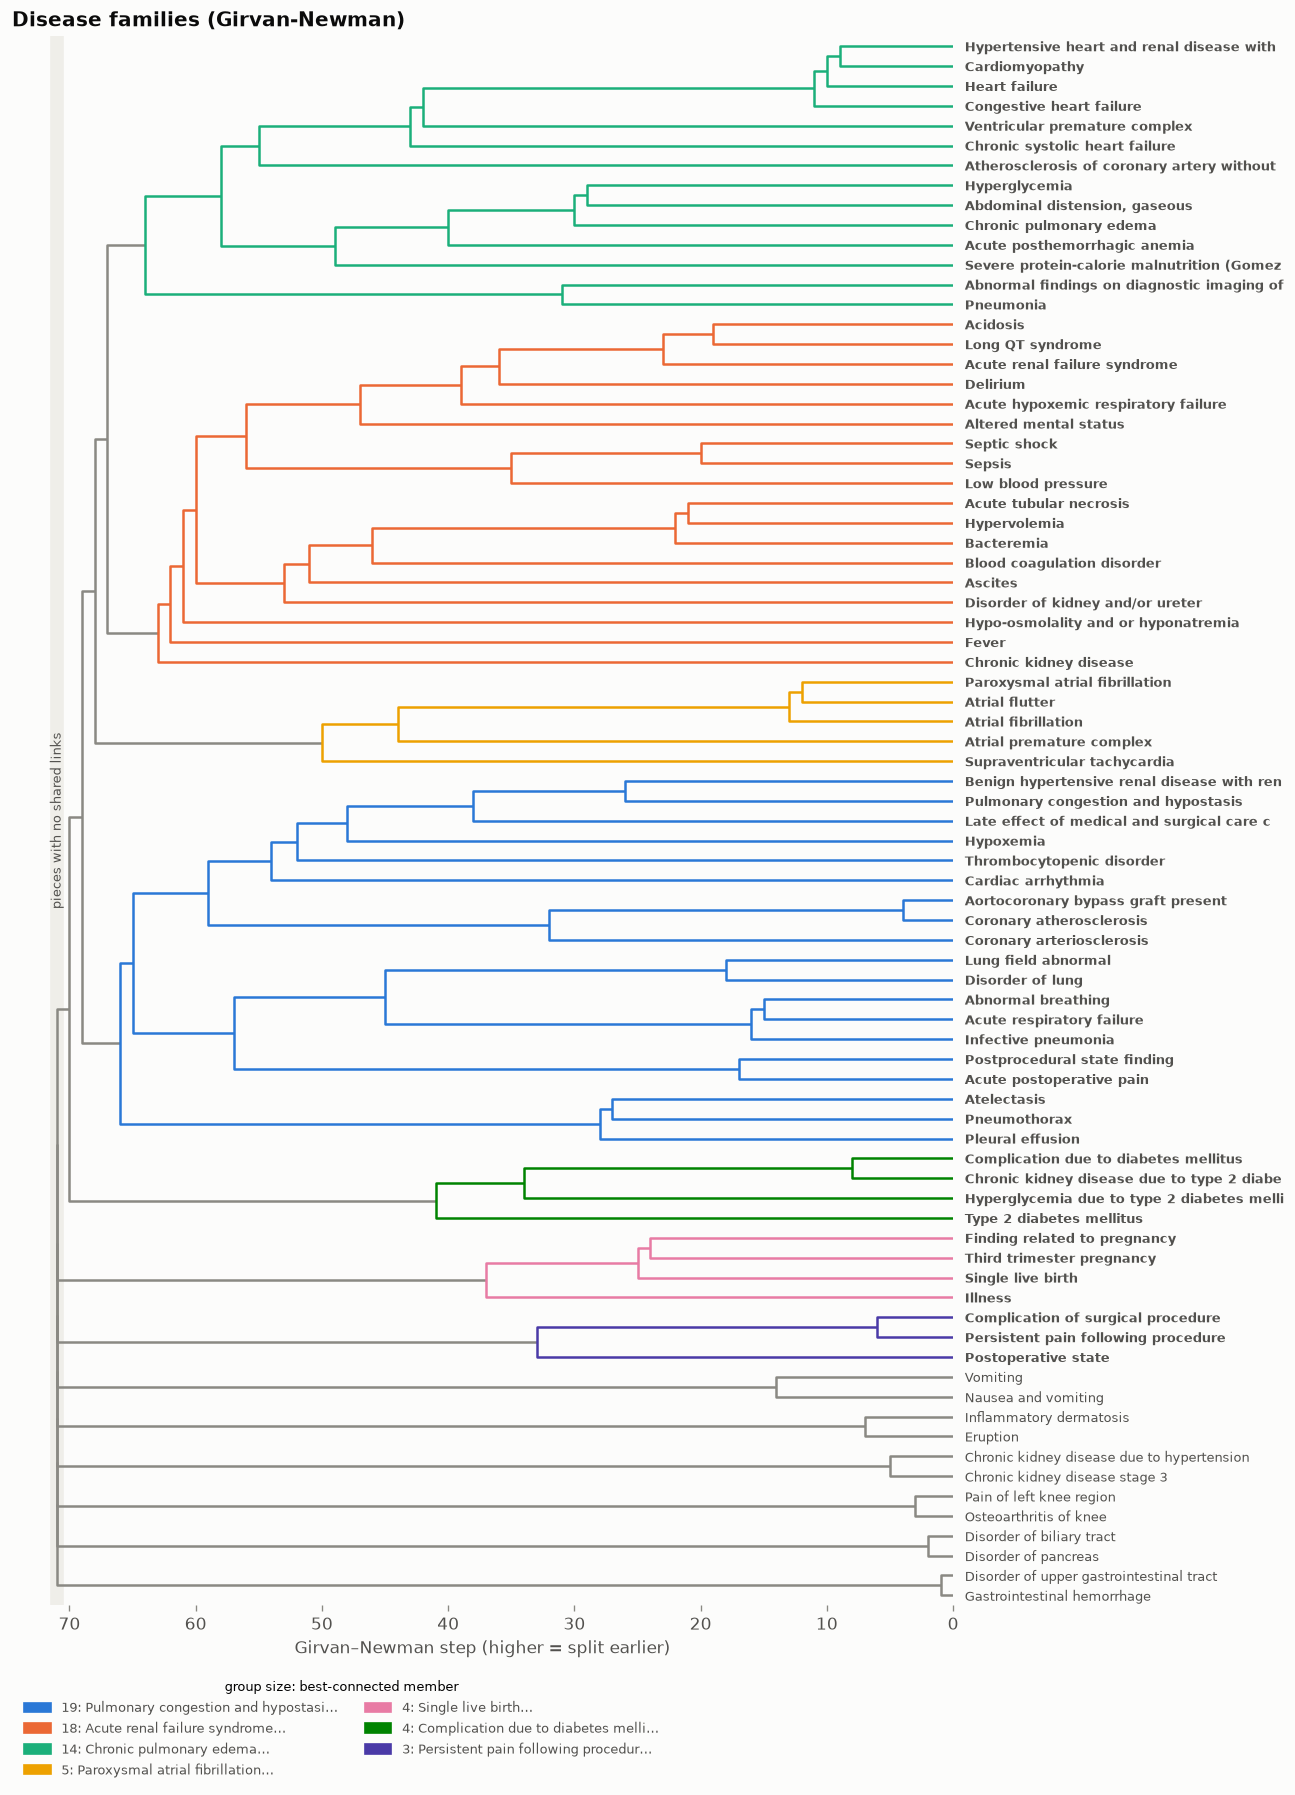
\includegraphics[width=0.85\textwidth]{04_disease_families.png}
\caption{Tree of splits for the diagnosis network built on standardised codes, coloured by the 13 groups at the best cut. The large groups are lung and breathing failure, sepsis and kidney failure, and heart failure.}
\label{fig:families}
\end{figure*}

\subsection{How things spread through the patient networks}

Finally, we simulate how a signal travels through the patient networks. This is a mathematical analogy, not a model of real infection, and shows how network shape affects how far information from one stay reaches. In the SIR model~\cite{kermack1927contribution}, each stay is susceptible, ``infected'', or recovered. We start from 10 random stays; at each step an infected stay passes the signal to each neighbour with probability 0.3 and recovers with probability 0.1. After 10 steps the signal has reached 27\% of stays in the honest long-stay network, 13\% in the cheating network, and 87\% in the random network (47\%, 31\%, and 90\% for high blood pressure; Figure~\ref{fig:spread}, left). Tight groups and long paths slow the spread; the random network, with short paths and almost no triangles, lets it reach nearly everyone quickly.

\begin{figure*}[!t]
\centering
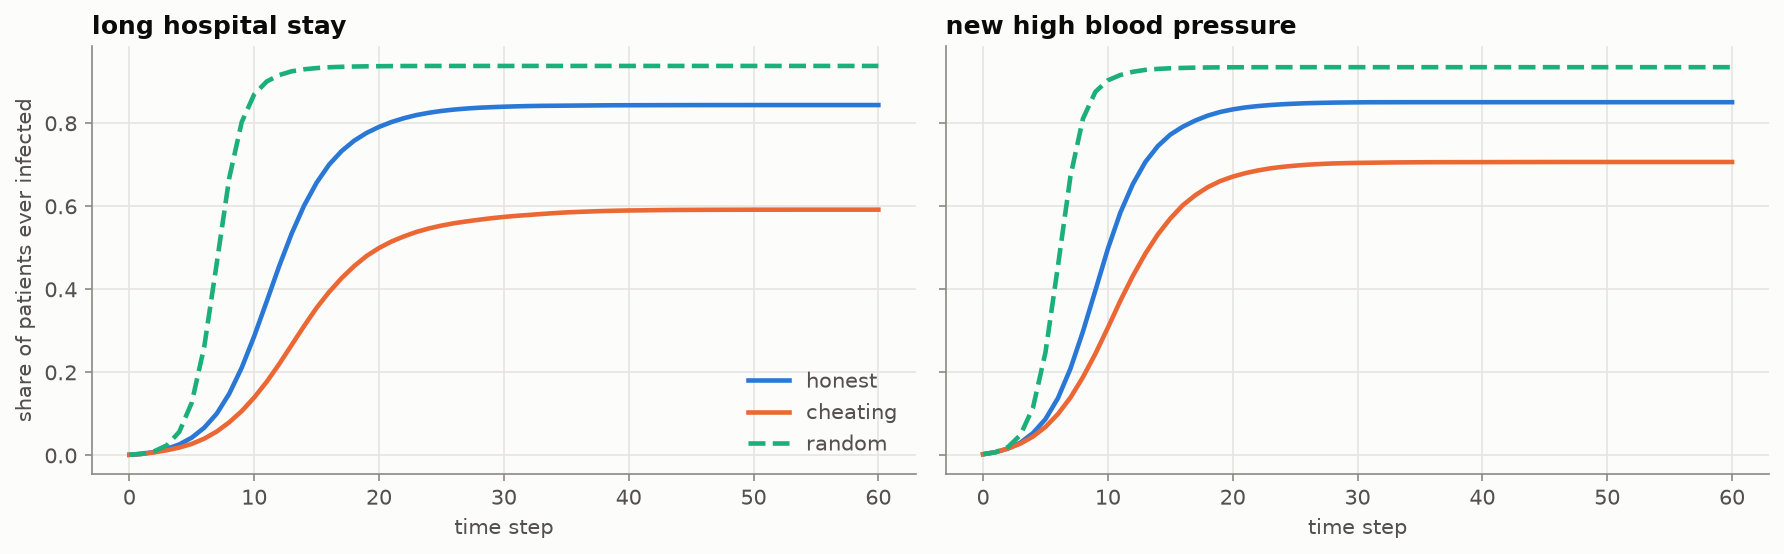
\includegraphics[width=0.49\textwidth]{05_sir_spreading.png}\hfill
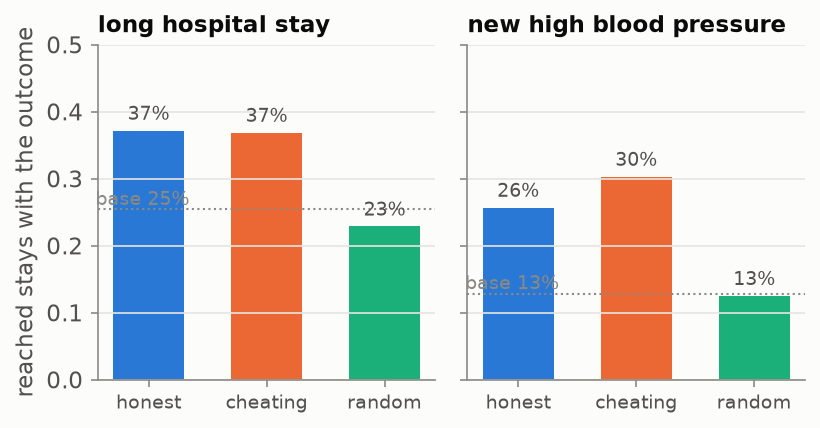
\includegraphics[width=0.49\textwidth]{05_cascade_reach.png}
\caption{Spreading through the patient networks. Left: share of stays ever reached in the SIR simulation over time (average of 20 runs). Right: share of stays reached by a cascade from positive stays that are themselves positive; the dotted line is the base rate.}
\label{fig:spread}
\end{figure*}

The independent cascade~\cite{kempe2003maximizing} asks a more clinical question. We start from a random 5\% of the stays \emph{with} the outcome, and each newly reached stay gets one chance to pass the signal to each neighbour (probability 0.1). Of the stays reached in the honest network, 37\% are long stays (base rate 25\%) and 26\% are high-blood-pressure cases (base rate 13\%); in the random network the reached stays match the base rate (Figure~\ref{fig:spread}, right). Following connections from known cases therefore leads to other likely cases. This is the idea behind label propagation, a simple way to make predictions from a network.

We also tried spectral partitioning~\cite{vonluxburg2007tutorial}, another way to split a network into groups. With 10 groups it finds much weaker structure than Leiden (modularity 0.41 against 0.93), but with as many groups as Leiden finds it nearly catches up (0.89). These networks have dozens of natural communities, not a few large ones.
